\section{Classificazione}
In questa parte si è classificato il dataset, al fine di predire in quali casi un lavoratore possa plausibilmente lasciare l’azienda o no (in termini più specifici, quale possa essere il valore della sua \textit{Attrition}). \\
Il metodo di classificazione \textit{Decision Tree} è quello che più di tutti fornisce risultati facilmente leggibili ed è stato quindi scelto per primo. Il carattere fortemente sbilanciato del dataset, in particolare in riferimento all’\textit{Attrition}, ha tuttavia, portato a risultati poco significativi. \\\\
Per ottenere un dataset più bilanciato, abbiamo allora applicato due tecniche di \textit{sampling}: il \textit{Random Undersampling}, che rimuove oggetti della classe maggioritaria (nel nostro caso \textit{Attrition} pari a \textit{No}) e la \textit{Synthetic Minority Oversampling Technique} (\textit{SMOTE}), che genera nuovi oggetti della classe in minoranza (con \textit{Attrition} pari a \textit{Yes}) osservando i preesistenti oggetti più simili.\\\\
Successivamente, abbiamo applicato ulteriori algoritmi di classificazione al dataset, per osservare un possibile aumento dell’accuratezza. Nello specifico, sono stati applicati l’algoritmo \textit{Random Forest} e\textit{ K-Nearest Neighbors} (KNN).

\subsection{Preparazione del dataset}
Il dataset in nostro possesso era già diviso in due parti: il \textit{training set} e il \textit{test set}. Dopo aver proceduto all’eliminazione dei valori mancanti in entrambi (con le procedure di cui abbiamo parlato sopra), abbiamo suddiviso il dataset di \textit{training}: il 70\% è stato destinato effettivamente al \textit{training}, mentre il restante 30\% ha formato il \textit{validation set}, necessario per confrontare fra loro tutti i modelli generati dall’addestramento sul \textit{training} al fine di trovare i parametri ottimali per i classificatori. \\\\Le tecniche di \textit{Oversampling} e \textit{Undersampling} sopra menzionate sono state applicate solo al \textit{training set }in senso stretto.

\subsection{Ottimizzazione dei parametri}
Per quanto riguarda i metodi di \textit{Decision Tree}, l’ottimizzazione dei parametri è stata eseguita applicando l’algoritmo di\textit{ random search} al \textit{training set} originale, sia prima che dopo l’applicazione dello \textit{SMOTE} o del \textit{Random Undersampling}. \\\\L’algoritmo ha addestrato diversi classificatori, testando di volta in volta diverse combinazioni dei parametri\textit{ Max Depth} (profondità massima dell’albero), \textit{Min Sample Split} (numero minimo di oggetti per procedere a una ramificazione) e \textit{Min Sample Leaf} (numero minimo di oggetti per foglia), oltre che possibili misure di impurità (indice di Gini o entropia).
\\\\Nella tabella \ref{tab:TabParametriDecisionTree} riportiamo ciascun parametro dei vari modelli e i relativi risultati: l’accuratezza, il punteggio F1 medio (ovvero, la media della media armonica di \textit{precision} e \textit{recall} per i due valori di \textit{Attrition}) e la curva di ROC (rapporto fra FP e TP). Tali risultati sono riportati sia per il \textit{training set} che per il \textit{validation set}.
\begin{table}[H]
\centering
\resizebox{0.99\textwidth}{!}{
\begin{tabular}{|l|S|S|S|S|S|S|}
\hline
            & \textbf{{Modello 1} }     & \textbf{{Modello 2}}      & \textbf{{Modello 3}}      & \textbf{{Modello 4}}      & \textbf{{Modello 5}}      & \textbf{{Modello 6} }     \\\hline
\textbf{Sampling}     & {Nessuno}     & {Nessuno}     & {\textit{SMOTE}}       & {\textit{SMOTE}}       &\begin{tabular}[c]{@{}c@{}}\textit{Random}\\ \textit{Undersampling}\end{tabular}  & \begin{tabular}[c]{@{}c@{}}\textit{Random}\\ \textit{Undersampling}\end{tabular}   \\
\hline
\textbf{Criterion}    & Gini        & Gini        & {Entropia}    & Gini        & Gini        & Gini        \\ 
\hline
\textbf{Min Sample Split} & 29          & 15          & 31          & 4           & 6           & 23           \\
\hline
\textbf{Min Sample Leaf } & 34          & 25          & 12          & 5           & 9           & 5            \\\hline
\textbf{Max Depth}    & 4           & 12          & 17          & 13          & 17          & 4              \\\hline
\textbf{Training Accuracy}      & 0,851388889 & 0,854166667 & 0,894648829 & 0,931438127 & 0,848360656 & 0,790983607       \\\hline
\textbf{Training F1-Score}  & 1,23507305  & 1,34876709  & 1,78861433  & 1,86287012  & 1,6964715   & 1,58038138                  \\  \hline     
\textbf{Training AUC-ROC}    & 0,594097812 & 0,644703657 & 0,894648829 & 0,931438127 & 0,848360656 & 0,790983607                    \\       \hline   
\textbf{Validation Accuracy}      & 0,844660194 & 0,851132686 & 0,815533981 & 0,763754045 & 0,692556634 & 0,724919094                            \\\hline
\textbf{Validation F1-Score} & 1,11397849  & 1,23989305  & 1,17272962  & 1,17489987  & 1,18883071  & 1,26164874                          \\\hline
\textbf{Validation AUC-ROC}      & 0,553801257 & 0,596041604 & 0,574640826 & 0,589531577 & 0,654108051 & 0,696572882              \\
\hline
\end{tabular}
}
\caption{Parametri, accuratezza, \textit{F1-score} e \textit{AUC-ROC} risultanti dalla \textit{RandomGridSearch} con diverse tecniche di \textit{sampling}}
\label{tab:TabParametriDecisionTree}
\end{table}
\noindent Nei modelli generati dall’algoritmo \textit{Decision Tree}, in media i risultati ottenuti con il \textit{training set} originale hanno valori di accuratezza di 85\% (Modelli 1 e 2). Si è notato un sensibile miglioramento applicando al \textit{training set} lo \textit{SMOTE} (Modelli 3 e 4). Con il \textit{Random Undersampling} non si sono ottenuti invece miglioramenti (Modello 5) e, in taluni casi (Modello 6), si è anzi constatata una diminuzione dell’accuratezza.\\\\
In tutti i modelli addestrati con \textit{SMOTE} o \textit{Random Undersampling} si nota una diminuzione dell’accuratezza sul \textit{validation set}. In fase di test i risultati dell’accuratezza (misurata sia tramite \textit{cross validation} impostata a 10, sia tramite \textit{accuracy score}) hanno confermato questo fenomeno: i modelli ottenuti con tecniche di \textit{sampling} soffrono così di \textit{overfitting}.
\begin{figure}[H]
	\centering
	\subfloat[] 
	{
		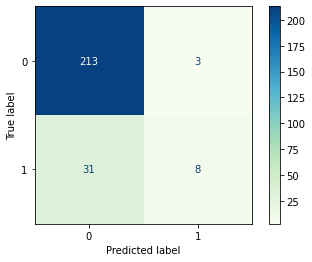
\includegraphics[width=.40\textwidth]{Immagini/MatriceM1.png}
		\label{MatriceM2}
	}
	\quad
	\subfloat[]
	{
		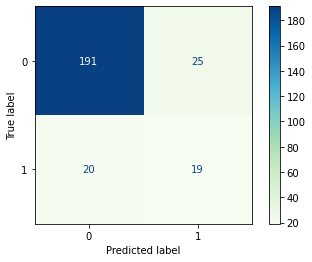
\includegraphics[width=.40\textwidth]{Immagini/MatriceM4.png}
		\label{MatriceM4}
    }
    \caption{Matrici di confusione ottenute applicando sul \textit{test set} il (a) \textit{Modello 1} e (b)\textit{ Modello 4}. Si può notare la difficoltà dei modelli nel riconoscimento corretto dei dipendenti con \textit{Attrition = 1}, ovvero i lavoratori che abbandonano la IBM.}
	\label{MatriciM1M4}
\end{figure}
\begin{figure}[H]
    \centering
    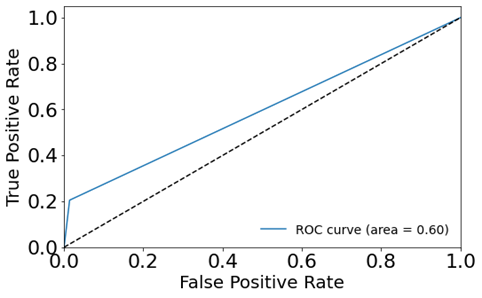
\includegraphics[width=0.45\textwidth]{Immagini/ROCM1.png}
    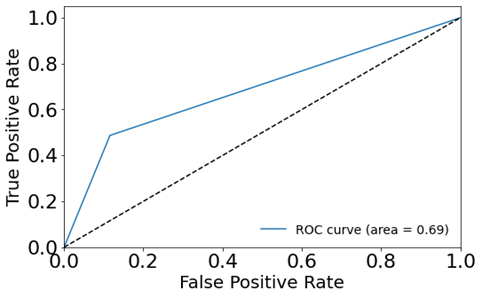
\includegraphics[width=0.45\textwidth]{Immagini/ROCM4.png}
    \caption{Differenti curve di ROC: Modello 1, Modello 4}
    \label{fig:ROC}
\end{figure}
   
\subsection{Altri modelli decisionali}
\begin{wraptable}{r}{70mm}
\centering
\vspace{-1.2cm}
\small
    \begin{tabular}{|c|S|S|}
        \hline
        K & \multicolumn{1}{c|}{\textbf{\begin{tabular}[c]{@{}c@{}}Accuratezza \\ train\end{tabular}}} & \multicolumn{1}{c|}{\textbf{\begin{tabular}[c]{@{}c@{}}Accuratezza \\ con SMOTE\end{tabular}}}\\ \hline
        1 & 0.7424804873405673 & 0.7567086834733894 \\ \hline
        2&0.8085760517799352&  0.7516176470588236 \\\hline
        3&0.7862364363221015&  0.7308263305322129 \\\hline
        4&0.8221682847896441& 0.7308263305322129\\\hline
        5&0.801770416904626&  0.7132703081232493\\\hline
        6&0.8241100323624595&  0.6973879551820729\\ \hline
        7&0.8124595469255663& 0.6923879551820729\\ \hline
        8&0.8279840091376356& 0.6882072829131654\\ \hline
        9&0.8241005139920045& 0.6731442577030813\\ \hline
        10&0.830906148867314& 0.6839705882352941\\ \hline
        11&0.8289644012944983& 0.6781652661064427\\ \hline
    \end{tabular}\setlength{\belowcaptionskip}{-20pt}
    \caption{Accuratezze di diversi KNN con diversi valori di K e \textit{training set}}
\end{wraptable}  

Come detto, sono stai poi applicati altri due algoritmi di classificazione. Il \textit{KNN}, basato sull’osservazione dei valori simili più vicini, ha richiesto lo \textit{scaling} delle varie \textit{\textit{feature}} del dataset. I valori migliori sono stati ottenuti impostando \textit{K} pari a 11 per il \textit{training set} originario e pari a 3 per quello espanso con lo \textit{SMOTE}. Tuttavia, sono risultati in linea con quelli degli alberi decisionali.
\\\\Risultati migliori sono stati invece generati dall’algoritmo \textit{Random Forest}, impostato per generare 100 diversi alberi. Come per gli alberi decisionali, le combinazioni migliori dei parametri sono stati impostate con l’ausilio del \textit{random search}.
\\\\Nella tabella \ref{RandomForest} vengono presentati i risultati ottenuti e una comparazione con due dei metodi ottenuti con gli alberi decisionali.

\begin{table}[H]
\vspace{1em}
\small
\centering
\begin{tabular}{|l|S|S|}
\hline
                          & \textbf{\begin{tabular}[c]{@{}c@{}}Modello \\ Random Forest 1\end{tabular}} & \textbf{\begin{tabular}[c]{@{}c@{}}Modello \\ Random Forest 2\end{tabular}} \\ \hline
\textbf{Sampling}         & {Nessuno}                                                                     & {SMOTE}                                                                       \\ \hline
\textbf{Criterion}        & {Gini, Gini, Gini}                                                            & {Entropia, Gini, Entropia}                                                    \\ \hline
\textbf{Min Sample Split} & {5, 5, 5}                                                                     & {5, 10, 20}                                                                   \\ \hline
\textbf{Min Sample Leaf}  & {1, 1, 5}                                                                     & {1, 1, 1}                                                                     \\ \hline
\textbf{Max Depth}        & {26, 14, 8}                                                                   & {27, 32, 19}                                                                  \\ \hline
\textbf{Train Accuracy}           & 0,973611111                                                                 & 0,987458                                                                    \\ \hline
\textbf{Train F1-Score}    & 1,8999177                                                                   & 1,974913                                                                    \\ \hline
\textbf{Train AUC-ROC}        & 0,922131148                                                                 & 0,987458                                                                    \\ \hline
\textbf{Validation Accuracy}          & 0,851132686                                                                 & 0,847896                                                                    \\ \hline
\textbf{Validation F1-Score}   & 1,23989305                                                                  & 1,286777                                                                    \\ \hline
\textbf{Validation AUC-ROC}          & 0,596041604                                                                 & 0,617106                                                                    \\ \hline
\end{tabular}
\caption{Modelli \textit{Random forest} (con i primi tre alberi) addestrati sul \textit{training set} e sul \textit{training set} su cui è stato applicato lo SMOTE}
\label{RandomForest}
\end{table}

\begin{table}[H]
\resizebox{0.99\textwidth}{!}{
\begin{tabular}{|c|c|c|c|c|}
\hline
                               & \textbf{Modello 1} & \textbf{Modello 4} & \textbf{\begin{tabular}[c]{@{}c@{}}Modello 1 Random\\ Forest\end{tabular}} & \textbf{\begin{tabular}[c]{@{}c@{}}Modello 2 Random \\ Forest (SMOTE)\end{tabular}} \\ \hline
\textbf{Training accuracy}     & 0,851            & 0,931            & 0,973                                                                    & 0,987                                                                             \\ \hline
\textbf{Validation accuracy}   & 0,844            & 0,763            & 0,851                                                                    & 0,847                                                                             \\ \hline
\textbf{Test Accuracy}         & 0.86             & 0.82             & 0.96                                                                     & 0.97                                                                              \\ \hline
\textbf{Cross-validation = 10} & 0.83             & 0.85             & 0.85                                                                     & 0.90                                                                              \\ \hline
\end{tabular}}
\caption{Confronto tra le accuratezze registrate con diversi modelli e diverse composizioni del \textit{training set}}
\end{table}
\noindent I risultati ottenuti sul \textit{training set}, sia per il dataset originario che per quello espanso, sono sensibilmente migliori di quelli offerti dagli alberi decisionali. Si nota anche qui tuttavia una diminuzione con il \textit{validation set}.
Con il \textit{test set}, invece, i due modelli si dimostrano particolarmente efficaci. In particolare il secondo, ottenuto con lo \textit{SMOTE}, ha fornito risultati estremamente positivi, anche osservando la curva di ROC.
\begin{figure}[H]
    \centering
    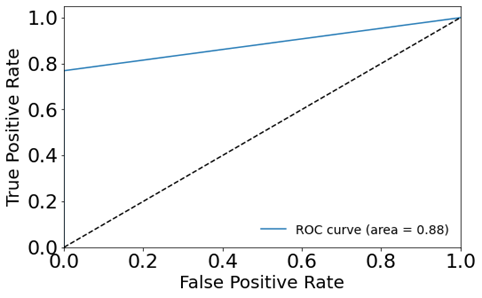
\includegraphics[width=0.45\textwidth]{Immagini/ROCR1.png}
    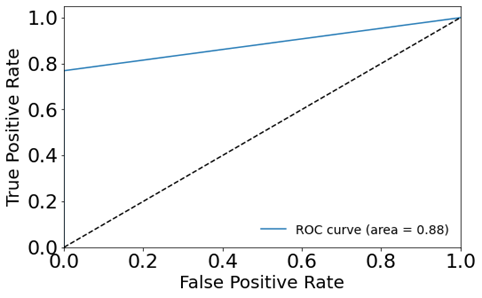
\includegraphics[width=0.45\textwidth]{Immagini/ROCR2.png}
    \caption{Differenti curve di ROC: Random Forest 1, Random Forest 2}
    \label{fig:ROC2}
\end{figure}
% \begin{figure}[H]
% 	\centering
% 	\subfloat[Curva di ROC ottenuta con random forest e addestramento su training set] 
% 	{
% 		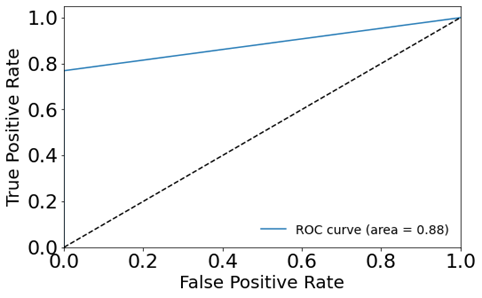
\includegraphics[width=.45\textwidth]{Immagini/ROCR1.png}
% 		\label{ROCRandomForest1}
% 	}
% 	\quad
% 	\subfloat[Curva di ROC ottenuta con random forest e addestramento su training set con SMOTE]
% 	{
% 		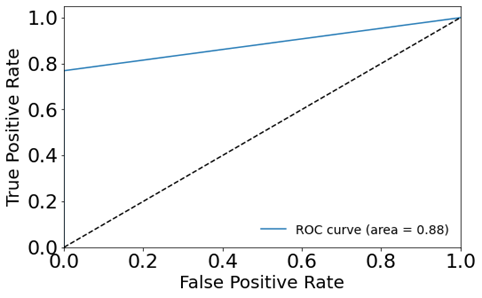
\includegraphics[width=.45\textwidth]{Immagini/ROCR2.png}
% 		\label{ROCRandomForest2}
%     }
% 	\label{ROCRandomForest}
% \end{figure}
Di seguito, il primo albero generato dal modello Random Forest 2.
\begin{figure}[H]
    \centering
    \small
    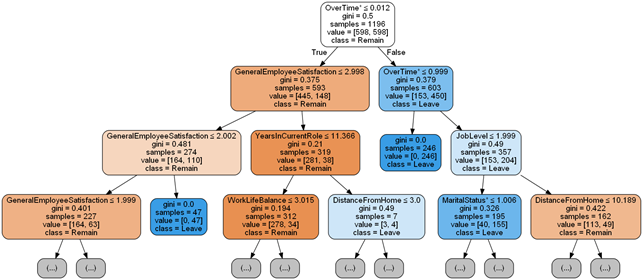
\includegraphics[scale=0.9]{Immagini/alberoRandomForest.png}
    \caption{Albero generato dall'algoritmo \textit{Random Forest}}
    \label{fig:alberoRandomForest}
\end{figure}
\noindent Dall’analisi dell’albero presentato, e dai pesi assegnati da ciascuno dei classificatori addestrati alle diverse \textit{\textit{feature}}, si rileva l’importanza di quattro parametri particolarmente rilevanti per individuare l'\textit{Attrition}: \textit{OverTime}, \textit{JobLevel}, \textit{DistanceFromHome} e \textit{GeneralEmployeeSatisfaction} (i primi tre da noi già utilizzati per il clustering). Meno rilevanti sono, ad esempio, \textit{Gender} e \textit{Age}. 
\\\\Nel caso specifico sopra, si nota, ad esempio, che i lavoratori con basso \textit{OverTime} tendono a rimanere in azienda. Maggiori valori di \textit{OverTime} portano invece all’abbandono dell’azienda, con l’eccezione di alcuni casi determinati da \textit{JobLevel} e \textit{DistanceFromHome}.
\\\\Ulteriori analisi richiederebbero una lettura dell’albero a una maggiore profondità: tuttavia, è da ricordare che quello sopra proposto è soltanto uno dei 100 alberi del \textit{Random Forest}.
\subsection{Conclusioni sulla classificazione}
In generale sono stati notati problemi legati alla natura estremamente sbilanciata del dataset, con una predominanza di oggetti con \textit{Attrition} pari a \textit{No}, che non hanno permesso ai classificatori di riconoscere correttamente i possibili lavoratori che abbandonano l’azienda. \\\\Risultati migliori sono stati ottenuti sul \textit{training set} con l’applicazione del metodo \textit{SMOTE}. Tali modelli non sono comunque risultati adeguati per il \textit{test set} (e il \textit{validation set}), soffrendo di \textit{overfitting}. Il problema si è presentato anche con il classificatore \textit{KNN}, mentre il \textit{Random Forest} ha costituito una valida soluzione, in quanto è un algoritmo nato con lo scopo di evitare le problematiche di \textit{overfitting} che affliggono i tradizionali classificatori basati su alberi di decisione. %applicando un diverso albero decisione a diverse sezioni dal dataset.

